\chapter{هم‌ایستایی یا هومئوستازی (Homeostasis)}
\section{ساز و کار هم‌ایستایی}
    هم‌ایستایی یا هومئوستازی
    \footnote{Homeostasis}
    در زیست‌شناسی به معنای حفظ پایداریِ محیط داخلی بدن و ثابت نگه داشتن شرایط فیزیکی و شیمیایی جاندار است. عملکرد بهینه جاندار در گرو این ویژگی است که متغیرهای زیادی از جمله دما و تعادل مایعات بدن را در محدوده‌ای از پیش تعیین شده نگه می‌دارد 
    (محدوده هومئوستاتیک). 
    پی‌اچِ مایعات برون‌سلولی، غلظت یون‌های سدیم، پتاسیم و کلسیم و سطح قند خون نیز بخشی از این متغیرهاست که پیوسته کنترل می‌شود. جاندار، علی‌رغم تغییرات محیط، نوع رژیم غذایی و مقدار فعالیت بدنی، تعادل متغیرهای بدنش را، هرکدام با یک یا چند سازوکار هومئوستاتیک به‌طوری پایدار حفظ می‌کند که تمام این فرایندهای تنظیمی باهم حیات را تدوام می‌بخشد. 
    پلاستیسیته هموستاتیک نیز در زمینه تولیدکننده الگوهای مرکزی بسیار مهم است. در این زمینه، خواص عصبی در پاسخ به تغییرات محیطی به منظور حفظ خروجی عصبی مناسب تعدیل می‌شوند.
    در این قسمت، اضافه کردن هر دو نوع این ساز و کار را به لایه دوم بررسی می‌کنیم. 
    \section{ساز و کار هم‌ایستایی براساس فعالیت}
    ابتدا، به عنوان اولین آزمایش، به یک شبکه ساده، این ساز و کار را اضافه کرده، و سپس به شبکه های بخش قبلی نیز آن را اضافه می‌کنیم. همانطور که در شکل 
    \ref{fig:part2-simple-stdp-homeostasis}
    نیز مشاهده می‌کنیم، اضافه کردن این ساز و کار به تنهایی به یک شبکه ساده با قانون یادگیری 
    STDP 
    توانسته است نسبت به حالت ساده، بهتر الگو ها را تشخیص دهد. هر چند با تکرار شبیه سازی، ممکن است این یادگیری انجام نشود چرا که ساز و کار هومئوستازی بیشتر در کنار ساز و کار های دیگر برای بهبود و حفظ پایداری می تواند کاربرد داشته باشد.

    \begin{figure}[!ht]
        \centering
        \includegraphics[width=0.95\textwidth]{plots/part2-simple-stdp-homeostasis.pdf} 
        \captionsetup{width=.9\linewidth}
        \caption{\textbf{اضافه کردن ساز و کار هومئوستازی براساس فعالیت به یک شبکه ساده.} همانطور که در شکل بالا نیز مشاهده می‌کنیم، اضافه کردن این ساز و کار به تنهایی برای یک شبکه ساده، می‌تواند نسبت به حالتی که وجود نداشته باشد، یادگیری را بهتر کن.(یادگیری زودتر اتفاق بیوفتد یا تعداد نورون های فعال برای الگو بیشتر شود) 
        اما این ساز و کار به تنهایی نمی‌تواند یادگیری مدل را تنظیم کند و بهتر است درکنار ساز و کار های دیگر شبکه مورد استفاده قرار گیرد.}
        \label{fig:part2-simple-stdp-homeostasis}
    \end{figure}

    حال این ساز و کار را به شبکه قسمت قبل که دارای ساز و کار های مهار جانبی و 
    k-winners-take-all 
    بود اضافه می‌کنیم. انتظار داریم که اضافه کردن این ساز و کار بتواند پایداری شبکه قبل را بهتر کند.
    همانطور که مطابق شکل 
    \ref{fig:part2-simple-stdp-kwta-lateral-inhibtion-homeostasis} 
    نیز مشاهده می‌کنیم، افزودن این ساز و کار به شبکه باعث می‌شود که شبکه توانایی یادگیری خود را حفظ کند و نسبت به قبل پایدار تر شود. در این مدل، ما پارامتر های ساز و کار هومئوستازی را به نحوی دادیم که در یک پنجره زمانی که ورودی داده می‌شود، فقط نصف نورون ها فعالیت داشته باشند. از این رو مطابق شکل نیز ملاحظه می‌کنیم که تعداد ضربه ها هنگامی که یک ورودی داده می‌شود نسبت به مدل های قبلی بیشتر شده است و گویی که نورون مخصوص به یک الگو، فقط و فقط در زمان ورودی دادن آن الگو فعال می‌شود.

    \begin{figure}[!ht]
        \centering
        \includegraphics[width=0.95\textwidth]{plots/part2-simple-stdp-kwta-lateral-inhibtion-homeostasis.pdf} 
        \captionsetup{width=.9\linewidth}
        \caption{\textbf{ ساز و کار، مهار جانبی، 
        k-winners-take-all و 
        هومئوستازی براساس فعالیت در یک شبکه.} همانطور که در شکل بالا نیز مشاهده می‌کنیم، اضافه کردن این ساز و کار هومئوستازی به شبکه قسمت قبل که هم مهار جانبی داشت و هم 
        k-winners-take-all 
        توانسته است الگوهای ورودی را به خوبی تشخیص دهد. همچنین ساز و کار هومئوستازی باعث شده که میزان فعالیت نورون ها در یک پنجره زمانی
        (در اینجا پنجره زمانی که ورودی داده می‌شود) 
        متعادل شود و ما شاهد فعالیت بیشتر نورون های لایه خروجی برای الگو متعلق به خود هستیم.}
        \label{fig:part2-simple-stdp-kwta-lateral-inhibtion-homeostasis}
    \end{figure}

    \subsection{افزایش تعداد الگو ها}
        حال در این مرحله، تعداد الگو های ورودی و در نتیجه تعداد نورون های خروجی را افزایش می‌دهیم. برای اینکار از مجموعه داده مخزن دانشگاه واترلو و همچنین یک عکس تصادفی
        (من در اینجا عکس خودم را به عنوان نمونه قرار داده ام)
        استفاده می‌کنیم.
        (شکل \ref{fig:part2-5-patterns})

        \begin{figure}[!ht]
            \centering
            % \begin{adjustbox}{minipage=\linewidth,scale=0.5}
                \begin{subfigure}[b]{0.17\textwidth}
                    \centering
                    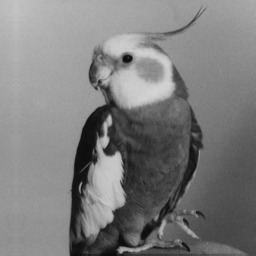
\includegraphics[width=\textwidth]{images/bird.jpg}
                    \caption{}
                    \label{fig:waterloo-bird}
                \end{subfigure}
                \hfill
                \begin{subfigure}[b]{0.17\textwidth}
                    \centering
                    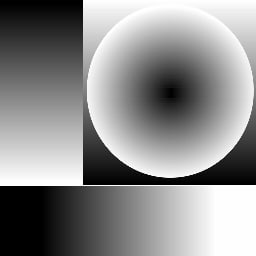
\includegraphics[width=\textwidth]{images/slop.jpg}
                    \caption{}
                    \label{fig:waterloo-slop}
                \end{subfigure}
                \hfill
                \begin{subfigure}[b]{0.17\textwidth}
                    \centering
                    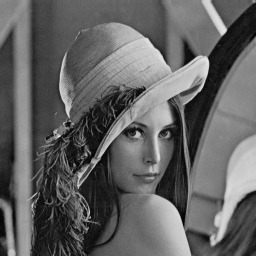
\includegraphics[width=\textwidth]{images/lena1.jpg}
                    \caption{}
                    \label{fig:waterloo-lena1}
                \end{subfigure}
                \hfill
                \begin{subfigure}[b]{0.17\textwidth}
                    \centering
                    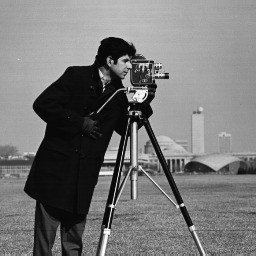
\includegraphics[width=\textwidth]{images/camera.jpg}
                    \caption{}
                    \label{fig:waterloo-camera}
                \end{subfigure}
                \hfill
                \begin{subfigure}[b]{0.17\textwidth}
                    \centering
                    
\includegraphics[width=\textwidth]{images/me.jpg}
                    \caption{}
                    \label{fig:extra-image}
                \end{subfigure}
            % \end{adjustbox}
            \caption{مجموعه داده مورد استفاده}
            \label{fig:part2-5-patterns}
        \end{figure}

        حال ساز و کار مورد نظر را به مدل اضافه می‌کنیم و مطابق شکل
        \ref{fig:part2-simple-stdp-kwta-lateral-inhibtion-homeostasis-more-patterns}
        ملاحظه می‌کنیم که مدل برای تعداد الگوهای بیشتر نیز می‌تواند توانایی خود در تشخیص آن ها را حفظ کند. حتی با تکرار شبیه سازی با دفعات زیاد نیز مدل همچنان در تشخیص الگو ها موفق بوده و پایداری خود را حفظ می‌کند. فقط دقت شود که به دلیل جلوگیری از شلوغی نمودار ها و تحلیل بهتر، در اینجا اندازه الگو های ورودی را کمی کاهش دادیم.

        \begin{figure}[!ht]
            \centering
            \includegraphics[width=\textwidth]{plots/part2-simple-stdp-kwta-lateral-inhibtion-homeostasis-5-patterns.pdf} 
            \captionsetup{width=.9\linewidth}
            \caption{\textbf{ ساز و کار، مهار جانبی، 
            k-winners-take-all و 
            هومئوستازی براساس فعالیت در یک شبکه: الگو های بیشتر} مطابق شکل ملاحظه می‌کنیم که مدل توانسته است از عهده تشخیص الگو های بیشتر نیز بربیاید. هر نورون توانسته است یکی از الگو ها را یاد بگیرد. در این آزمایش، با تکرار شبیه سازی، پایداری مدل حفظ می‌شود و هر نورون لایه خروجی، یک الگو را تشخیص می‌دهد.}
            \label{fig:part2-simple-stdp-kwta-lateral-inhibtion-homeostasis-5-patterns}
        \end{figure}
    \subsection{نتایج}
        حال که با ساز و کار هم‌ایستایی به عنوان ساز و کاری که میزان فعالیت نورون ها را در یک بازه زمانی کنترل می‌کند آشنا شدیم، ممکن است به این فکر کنیم که این ساز و کار چقدر می‌تواند کارایی مدلمان را نسبت به بخش قبل بهبود دهد. خوشبختانه مطابق شکل 
        \ref{fig:part1-evaluation-simple-stdp-LI-KWTA}
        ملاحظه می‌کنیم که توانایی مدل در تشخیص الگو ها به میزان قابل توجهی افزایش یافته است.

        \begin{figure}[!ht]
            \centering
            \begin{adjustbox}{minipage=\linewidth,scale=1}
                \begin{subfigure}[b]{0.5\textwidth}
                    \centering
                    \includegraphics[width=\textwidth]{plots/with-normalization/part1-evaluation-simple-stdp-LI-KWTA-Homeostasis-2-patterns.pdf}
                    \caption{2 الگو}
                    \label{fig:part1-evaluation-simple-stdp-LI-KWTA-2-patterns}
                \end{subfigure}
                \hfill
                \begin{subfigure}[b]{0.5\textwidth}
                    \centering
                    \includegraphics[width=\textwidth]{plots/with-normalization/part1-evaluation-simple-stdp-LI-KWTA-Homeostasis-10-patterns.pdf}
                    \caption{6 الگو}
                    \label{fig:part1-evaluation-simple-stdp-LI-KWTA-4-patterns}
                \end{subfigure}
                \vfill
                \begin{subfigure}[b]{0.5\textwidth}
                    \centering
                    \includegraphics[width=\textwidth]{plots/with-normalization/part1-evaluation-simple-stdp-LI-KWTA-Homeostasis-20-patterns.pdf}
                    \caption{20 الگو}
                    \label{fig:part1-evaluation-simple-stdp-LI-KWTA-6-patterns}
                \end{subfigure}
                \hfill
                \begin{subfigure}[b]{0.5\textwidth}
                    \centering
                    \includegraphics[width=\textwidth]{plots/with-normalization/part1-evaluation-simple-stdp-LI-KWTA-Homeostasis-30-patterns.pdf}
                    \caption{30 الگو}
                    \label{fig:part1-evaluation-simple-stdp-LI-KWTA-15-patterns}
                \end{subfigure}
            \end{adjustbox}
            \caption{\textbf{آزمایش مدل با تعداد الگو های متفاوت.}در این آزمایش یک مدل ترین شده روی الگو ها را، به اندازه یک بار ورودی دادن همه الگو ها شبیه سازی می‌کنیم. 
            (تعداد باری که هر الگو را مدل دیده است در هر آزمایش برابر است.) 
            مطابق شکل مشاهده می‌کنیم که مدل حتی توانسته است تا ۳۰ الگو را به طور کامل یاد بگیرد و با تکرار آزمایش نیز در یادگیری موفق است. مشاهده می‌کنیم که مشکلی که در مدل قبلی 
            (مدل شامل مهار جانبی و 
            k-winners-take-all) 
            باعث می‌شد برخی نورون ها فعالیتی از خود نشان ندهند و در نتیجه برخی الگو ها تشخیص داده نشوند، با اضافه شدن هم‌ایستایی مبتنی بر فعالیت رفع شده است. چرا که در این ساز و کار، ما میزان فعالیت نورون ها را کنترل می‌کنیم و نمی‌گذاریم که از حدی کمتر شود 
            (یک نورون هیچ الگوی را تشخیص ندهد) 
            یا از حدی بیشتر شده که یک نورون به ازای دو ورودی ضربه بزند.
            من این آزمایش را برای تعداد بیشتر الگو ها هم انجام دادم ولی به دلیل محدودیت زمان و منابع محاسباتی، و همچنین شلوغ شدن تصاویر، تا ۳۰ الگو را در اینجا آورده‌‌ام.}
            \label{fig:part1-evaluation-simple-stdp-LI-KWTA}
        \end{figure}




\clearpage
\section{ساز و کار هومئوستازی براساس ولتاژ (امتیازی)}
        حال در این قسمت، ساز و کار هومئوستازی براساس ولتاژ را به مدل اضافه می‌کنیم. کلیت مفهوم این ساز و کار نیز همانند ساز و کار قبلی است، اما تفاوت آن در چیزی است که آن را حفظ می‌کند. در این ساز و کار، سعی می‌شود که ولتاژ نورون را در محدوده‌ای که به عنوان پارامتر می‌گیرد، تنظیم کند. ابتدا این ساز و کار را به تنهایی و به همراه ساز و کار های دیگر به شبکه اضافه می‌کنیم و در نهایت آن را با نوع قبلی هومئوستازی مقایسه می‌کنیم. مطابق شکل 
        \ref{fig:part2-simple-stdp-voltage-homeostasis} 
        مشاهده می‌کنیم که افزودن ساز و کار هومئوستازی بر پایه ولتاژ توانسته است مدل را قادر سازد الگو های ورودی را تشخیص دهد. نکته جالبی که در این آزمایش وجود داشت این است که حتی با تکرار آزمایش نیز ،مدل به احتمال بیشتری نسبت به حالتی که ساز و کاری وجود نداشت تونایی خود در تشخیص الگو ها را حفظ می‌کرد.

        \begin{figure}[!ht]
            \centering
            \includegraphics[width=0.95\textwidth]{plots/part2-simple-stdp-voltage-homeostasis.pdf} 
            \captionsetup{width=.9\linewidth}
            \caption{\textbf{ اضافه کردن ساز و کار
            هومئوستازی براساس ولتاژ در یک شبکه ساده.} مطابق شکل ملاحظه می‌کنیم که با اضافه کردن این ساز و کار نیز، مدل توانسته است الگو های ورودی را تشخیص دهد. هر چند هنوز نیز با تکرار آزمایش مدل ممکن است در تشخیص الگو ها گاهی ناموفق باشد، ولی نسبت به حالتی که شبکه ساز و کاری ندارد شاهد پایداری بیشتری هستیم.}
            \label{fig:part2-simple-stdp-voltage-homeostasis}
        \end{figure}

        حال که تاثیر این ساز و کار را بر مدل ملاحظه کردیم، به سراغ اضافه کردن آن به شبکه‌ای که در نهایت در بخش دوم ساخته شد می‌رویم. همانطور که در شکل 
        \ref{fig:part2-simple-stdp-kwta-lateral-inhibition-voltage-homeostasis} 
        نیز ملاحظه می‌کنیم، اضافه کردن این ساز و کار به شبکه نیز مانند قسمت قبل است و مدل توانسته است الگو ها را تشخیص دهد. نکته‌ای که در مقایسه این ساز و کار با ساز و کار قبلی وجود دارد این است که ما در ساز و کار قبلی شاهد بودیم که در پنجره زمانی که ورودی ها داده می‌شدند، فعالیت نورون های لایه خروجی متراکم تر بود در حالی که چنین چیزی را در اینجا شاهد نیستیم.

        \begin{figure}[!ht]
            \centering
            \includegraphics[width=0.95\textwidth]{plots/part2-simple-stdp-kwta-lateral-inhibition-voltage-homeostasis.pdf} 
            \captionsetup{width=.9\linewidth}
            \caption{\textbf{ ساز و کار، مهار جانبی، 
            k-winners-take-all و 
            هومئوستازی براساس ولتاژ در یک شبکه.} همانطور که در شکل بالا نیز مشاهده می‌کنیم، اضافه کردن این ساز و کار هومئوستازی به شبکه قسمت قبل که هم مهار جانبی داشت و هم 
            k-winners-take-all 
            توانسته است الگوهای ورودی را به خوبی تشخیص دهد. همچنین ساز و کار هومئوستازی باعث شده که میزان فعالیت نورون ها در یک پنجره زمانی
            (در اینجا پنجره زمانی که ورودی داده می‌شود) 
            متعادل شود و ما شاهد فعالیت بیشتر نورون های لایه خروجی برای الگو متعلق به خود هستیم.}
            \label{fig:part2-simple-stdp-kwta-lateral-inhibition-voltage-homeostasis}
        \end{figure}

        \subsection*{مقایسه پیاده سازی}
            در این قسمت می‌خواهیم پیاده سازی دو ساز و کار را با یکدیگر مقایسه کنیم.
            \paragraph*{هومئوستازی مبتنی بر فعالیت} در هومئوستازی مبتنی بر فعالیت، تنظیم سطح فعالیت نورون ها بر اساس رفتار spiking آنها در یک پنجره زمانی تعریف شده طراحی شده است. این رفتار، یک پارامتر به نام 
            \texttt{activity\_rate} 
            دریافت می‌کند که نشان دهنده نرخ ضربه زدن نورون ها در پنجره زمانی مورد نظر است. این پنجره زمانی نیز خود با یک پارامتر به نام 
            \texttt{window\_size} مقدار دهی می‌شود. 
            همچنین یک پارامتر به نام 
            \texttt{updating\_rate} 
            نیز گرفته می‌شود که عامل مقیاس‌پذیری برای به‌روزرسانی آستانه‌های نورون‌ها است. علاوه بر آن پارامتر 
            \texttt{decay\_rate} 
            نیز وجود دارد تا نرخ به‌روزرسانی را در طول زمان کاهش می‌دهد تا تغییرات ممکن را تثبیت کند.
            نحوه کارکرد این ساز و کار به این صورت است که ضربه ها را در یک پنجره مشخص جمع می کند و آستانه نورون را بر اساس انحراف از فعالیت هدف تنظیم می کند. اگر فعالیت خیلی زیاد باشد، آستانه افزایش می یابد و اگر خیلی کم باشد، کاهش می یابد. به‌روزرسانی آستانه‌ها با 
            \texttt{updating\_rate} 
            مقیاس‌بندی می‌شود، و این نرخ پس از هر پنجره با 
            \texttt{updating\_rate} 
             تغییر می‌کند.
            
            \paragraph*{هومئوستازی مبتنی بر ولتاژ}
            این ساز و کار ولتاژ نورون ها را تنظیم می کند تا آن را در محدوده دلخواه نگه دارد. برای هدایت تنظیمات خود از آستانه های ولتاژ هدف، حداقل
            (\texttt{min\_ta})
            و حداکثر
            (\texttt{max\_ta})
            استفاده می کند. همچنین یک پارامتر 
            \texttt{eta\_ip} 
            نیز وجود دارد که مربوط به قدرت یا نرخ تنظیمی است که تغییرات در آن اعمال می شود. این ساز و کار بررسی می‌کند که آیا ولتاژ نورون از آستانه‌های تعیین‌شده فراتر می‌رود یا از آن پایین‌تر می‌آید و بر این اساس تنظیم می‌کند. تنظیمات به طور مستقیم از ولتاژ نورون کم می شود، 
            (تحت تاثیر پارامتر 
            \texttt{eta\_ip}).

            \paragraph*{مقایسه}
            \begin{itemize}
                \item \textbf{تمرکز:}هومئوستازی مبتنی بر فعالیت بر روی سطح فعالیت 
                (نرخ زدن) 
                نورون ها تمرکز دارد، در حالی که هومئوستازی مبتنی بر ولتاژ بر حفظ ولتاژ نورون در محدوده های خاص تمرکز دارد.
                \item \textbf{تطبیق پذیری:} هومئوستازی مبتنی بر فعالیت دارای یک نرخ تطبیقی ​​است 
                (\texttt{updating\_rate}
                که با 
                \texttt{decay\_rate} 
                به‌روزرسانی می شود)، 
                که می تواند آن را پویاتر کند و به تغییرات طولانی مدت در رفتار نورون پاسخ دهد. هومئوستازی مبتنی بر ولتاژ از یک نرخ ثابت 
                (\texttt{eta\_ip}) 
                استفاده می کند، که ممکن است در طول زمان کمتر به تغییرات پاسخ دهد مگر اینکه به صورت دستی تنظیم شود. 
                (این مورد را زمانی که شبیه سازی را تا مراحل بیشتری ادامه می‌دهیم شاهد هستیم. شکل 
                \ref{fig:part2-simple-stdp-kwta-lateral-inhibition-voltage-homeostasis} 
                را ببینید.)
                \item \textbf{پیچیدگی:} رویکرد مبتنی بر فعالیت به دلیل نیاز به شمارش ضربه ها و محاسبه به روزرسانی ها ممکن است به طور بالقوه پیچیده تر باشد. رویکرد مبتنی بر ولتاژ مستقیماً ولتاژ جریان را با محدوده‌های تنظیم شده مقایسه می‌کند، که ممکن است از نظر محاسباتی ساده‌تر باشد.
                \item \textbf{کاربرد:} انتخاب بین این روش ها به نیازهای خاص شبیه سازی بستگی دارد. به عنوان مثال، اگر تمرکز بر پایداری شبکه در برابر تغییرات ناگهانی در فعالیت ضربه ها باشد، روش مبتنی بر فعالیت ممکن است ترجیح داده شود. اگر اطمینان از عملکرد نورون‌ها در محدوده ولتاژ حیاتی‌تر باشد (احتمالاً برای جلوگیری از اشباع یا نورون‌های غیرفعال)،
                 روش مبتنی بر ولتاژ مناسب‌تر خواهد بود.
                 (مثلا هنگامی که یک جریان یا فعالیت زمینه داریم.)
            \end{itemize}

\clearpage
\section{(امتیازی) آزمایش با نسبت های مختلف الگو ها و لایه خروجی}
    در این قسمت، آزمایش را به ازای نسبت های مختلف تعداد نورون های لایه خروجی و تعداد الگو ها انجام می‌دهیم. در حالت کلی، سه حالت داریم:
    \begin{itemize}
        \item تعداد الگو ها بیشتر از تعداد نورون های لایه خروجی باشد
        \item تعداد الگو ها با نورون های لایه خروجی برابر باشد.
        (این آزمایش به صورت ضمنی در بخش های قبل انجام شد)
        \item تعداد الگو ها کمتر از تعداد نورون های لایه خروجی باشد
    \end{itemize}

    ابتدا حالتی را بررسی می‌کنیم که تعداد الگو ها کمتر از تعداد نورون های لایه خروجی باشد. برای این آزمایش، از یک شبکه با دو لایه و یک سیناپس از لایه ورودی به خروجی که از قانون یادگیری 
    STDP 
    استفاده می‌کند و همچنین ساز و کار مهار جانبی و 
    k-winners-take-all 
    دارد استفاده می‌کنیم. ساز و کار هومئوستازی مبتنی بر فعالیت نیز در لایه خروجی استفاده می‌شود. مطابق شکل 
    \ref{fig:part2-simple-stdp-kwta-lateral-inhibtion-homeostasis-more-patterns} 
    مشاهده می‌کنیم که در این حالت، در ابتدا بعضی نورون ها به ازای دو الگو ضربه می‌زنند و رفته رفته برای یکی از این دو الگو حساس تر شده و فقط هنگامی که آن الگو ورودی داده می‌شود فعال می‌شوند.


    \begin{figure}[!ht]
        \centering
        \includegraphics[width=0.95\textwidth]{plots/part2-simple-stdp-kwta-lateral-inhibtion-homeostasis-more-patterns.pdf} 
        \captionsetup{width=.9\linewidth}
        \caption{\textbf{ ساز و کار، مهار جانبی، 
        k-winners-take-all و 
        هومئوستازی مبتنی بر فعالیت: تعداد الگو ها ۵ عدد و تعداد نورون های خروجی ۳ عدد است.} مطابق شکل مشاهده می‌کنیم که در این حالت، در مراحل اولیه شبیه سازی بعضی از نورون های لایه خروجی به ازای دو الگو فعال می‌شوند و هر چه مراحل بیشتری می‌گذرد نسبت به یکی از این دو الگو حساس تر شده و در نهایت فقط هنگامی که آن الگو ورودی داده می‌شود ضربه می‌زنند.}
        \label{fig:part2-simple-stdp-kwta-lateral-inhibtion-homeostasis-more-patterns}
    \end{figure}

    حال آزمایش را برای حالتی که تعداد الگو ها از تعداد نورون های لایه خروجی کمتر است تکرار می‌کنیم و نتیجه را بررسی می‌کنیم. در این حالت مطابق شکل 
    \ref{fig:part2-simple-stdp-kwta-lateral-inhibtion-homeostasis-more-neurons}
    مشاهده می‌کنیم که بیشتر بودن تعداد نورون ها نسبت به الگو ها باعث می‌شود که به اندازه تعداد الگو ها، نورون های خروجی به الگو های متناظر حساس شوند و نورون های دیگر نیز ممکن است به یک الگوی دیگر مجددا حساس شده یا کلا ضربه‌ای نزنند و غیر فعال شوند.

    \begin{figure}[!ht]
        \centering
        \includegraphics[width=0.95\textwidth]{plots/part2-simple-stdp-kwta-lateral-inhibtion-homeostasis-more-neurons.pdf} 
        \captionsetup{width=.9\linewidth}
        \caption{\textbf{ ساز و کار، مهار جانبی، 
        k-winners-take-all و 
        هومئوستازی مبتنی بر فعالیت: تعداد الگو ها ۵ عدد و تعداد نورون های خروجی ۷ عدد است.} مطابق شکل مشاهده می‌کنیم که بیشتر بودن تعداد نورون ها نسبت به الگو ها باعث می‌شود که به اندازه تعداد الگو ها، نورون های خروجی به الگو های متناظر حساس شوند و نورون های دیگر نیز ممکن است به یک الگوی دیگر مجددا حساس شده یا کلا ضربه‌ای نزنند و غیر فعال شوند.}
        \label{fig:part2-simple-stdp-kwta-lateral-inhibtion-homeostasis-more-neurons}
    \end{figure}